\documentclass[11pt]{article} 
\usepackage{graphicx} 
\usepackage[authoryear,round]{natbib} 
\usepackage{caption}
\usepackage{subcaption}
\usepackage[mathlines]{lineno} 
\usepackage{setspace} 
\usepackage{mathrsfs} 
\usepackage{rotating} 
\usepackage{hyperref}
\usepackage{url} 
\usepackage{amssymb} 
\usepackage{multirow} 
\usepackage[none]{hyphenat} 
\usepackage{verbatim} 
\usepackage{amsmath}
\usepackage{threeparttable}
\DeclareGraphicsExtensions{.pdf,.png,.jpg} 
\setlength{\topmargin}{-.5in}  
\setlength{\textheight}{9in} 
\setlength{\oddsidemargin}{.125in} 
\setlength{\textwidth}{6.25in} 
\doublespacing 


\usepackage{array}
\newcolumntype{L}[1]{>{\raggedright\let\newline\\\arraybackslash\hspace{0pt}}m{#1}}
\newcolumntype{C}[1]{>{\centering\let\newline\\\arraybackslash\hspace{0pt}}m{#1}}
\newcolumntype{R}[1]{>{\raggedleft\let\newline\\\arraybackslash\hspace{0pt}}m{#1}}

\begin{document}
\begin{linenumbers}
\renewcommand\linenumberfont{\normalfont\small}
\setlength\linenumbersep{1cm}

\renewcommand{\theequation}{S3-\arabic{equation}}
 
% redefine the command that creates the equation no. 
\setcounter{equation}{0}  % reset counter 
\section*{Supplementary Information S3 - Model details for simulating a co-evolving resource-consumer metacommunity}
We model a $P$ patch meta-community where each patch is linked by migration to its neighboring patch. Within each patch, individuals of  the consumer species $C$ interact with individuals of the resource species $R$. We model coevolutionary dynamics in systems where consumers with a given phenotypic value are most effective at exploiting resources with a particular resource trait value, but may be poor at exploiting resources with other trait values (i.e., phentoypic matching - e.g., \citealt{nuismer07}). For instance, an herbivorous insect may evolve specific enzymes permitting it to exploit a novel plant resource, while the plant species may evolve alternative chemical defenses against the herbivore (\citealt{rasmann11a}). Alternatively, the ability of a resource to defend itself, and the ability of a consumer to exploit the resource, may itself be a composite trait of many distinct phenotypes (e.g., behavioral as well as morphological defenses), with consumer individuals varying in their ability to exploit different facets of resource defense (e.g., some consumers may be particularly good at identifying resource hiding sites, while others may have greater ability to puncture resource defenses such as shells).

In our model, the potential individual fecundity $w_{F,C}(t)$ of an individual consumer varies over time. An individual's breeding value determines the genetic component of this trait. $w_{F,C}(t)$ is also affected by how successfully an individual consumer is able to exploit the resource species. A consumer's ability to successfully exploit the resource, in turn, depends on two quantities: first, the individual's genetically determined exploitation ability, $\alpha$, and second, the phenotypic distribution of a resource defense trait $\delta$.  This adds a further source of genetic variation in individual fecundity, as well as an environmental effect that varies according to the prevailing distribution of the resource's phenotypes. At a given time $t$, the consumer's fecundity can be given by:

\begin{align}
w_{F,C}(t) &= \xi k \int_{y \in \{\delta\}} \frac{\exp(-(\alpha-y)^2)}{1 + \exp(-(\alpha-y)^2)} dy, \label{eqn:consumer_fecundity}
\end{align}
where $\xi$ is the breeding value characterizing the consumer's baseline fecundity and $k$ scales the effect of the interaction on consumers (it could thus represent, e.g., something like a conversion efficiency). Figure S3-A illustrates the per-capita effect of encounters between a given consumer and resource individual based on their phenotypic values. We note that removing the squared expression inside the exponential would describe a consumer-resource interaction with monotonic arms-race dynamics. 

The consumer's per-capita mortality rate $w_{M,C}$ is assumed to be constant during an individual consumer's's life; thus, we do not model reduction in survivorship through a failure to acquire resources (e.g., via starvation).  

Encounters with consumers are assumed to increase the mortality risk of the resource; we describe changes in the resource's mortality rate $w_{M,R}$ to depend on the extent to which the resource's trait is dissimilar to the distribution of consumer exploitation traits:

\begin{align}
w_{M,R}(t) &=  \gamma v \int_{x \in \{\alpha\}} \frac{\exp(-(x-\delta)^2)}{1 + \exp(-(x - \delta)^2)} dx,\label{eqn:resource_mortality}
\end{align}
where $\gamma$ is the breeding value characterizing the resource's baseline survivorship and $v$ scales the effect of the interactions on resource mortality.

We also model implicit exploitative competition among resource individuals. The outcome of such resource-resource competition determines the distribution of resource fecundities. We assume that the the resource's ability to defend itself against consumers comes at a cost to reproduction. Such a trade-off could arise, for instance, if energetic reserves need to be allocated to producing secondary compounds instead of fruit (e.g., \citealt{bazzaz87}; also \citealt{bohannan97}). Changes to resource fecundity are then modeled as:

\begin{align}
w_{F,R}(t) &= w_{F,R}(t) n_i \exp(-\rho \alpha^2),
\label{eqn:resource_fecundity}
\end{align}
where $n_i$ describes the aggregate effect of any encounters a resource individual $i$ may have with other resource individuals, and $\rho$ describes the severity of the trade-off between resource defense and resource fecundity. This entails that greater investment by the resource in any given anti-consumer strategy can entail greater fecundity costs.

Eqns. (\ref{eqn:consumer_fecundity} - \ref{eqn:resource_fecundity}) are mathematical abstractions in which a given individual of the focal species is assumed to encounter all possible individuals in the other species. In nature, however, encounters between individuals often result from Poisson processes (e.g., \citealt{hassell78}). Therefore, to capture the effects of contingent interspecific interactions on trait evolution, for a given individual of either species we instead simulate a random subset of possible encounters out of all possible species. The specific life history traits therefore change according to the cumulative interactions an individual experiences during a given time step, rather than summing over all possible interactions.

For the simulations of this model reported in the main text, we assumed that the phenotype governing consumer exploitation ability is controlled by three loci which we assume have additive effects on the consumer trait of interest. Similarly, the resource's defensive trait was assumed to be additively controlled by five loci. For both the consumer and resource species, genetic variations in the life history traits at birth were assumed to be minimal.

Figure S3-A illustrate how the strength $\rho$ of the tradeoff between resource defense and resource fecundity can govern the eco-evolutionary outcome of consumer-resource coevolution. When the tradeoff is weak, the resource can readily evolve anti-consumer defenses and drive the consumer extinct; when the tradeoff is strong, the resource can ill-afford to invest too heavily in a particular strategy and thus the manner in which it avoids predation shifts, enabling coevolutionary cycling. The consumer can only persist when the tradeoff faced by the resource is weak when there is sufficient migration from patches in which the tradeoff is strong. Figure S3-B show how the extent of migration between patches governs consumer persistence. Figure S3-B shows how when there is limited, the consumer population struggles to persist. However, when cross patch dispersal is relatively high, the inflow of maladapted consumers prevents successful local adaptation and consumer persistence is somewhat more limited. The parameter values used in the simulations of this model employed in the main text are available at \nolinkurl{https://github.com/kewok/spegg}.

\end{linenumbers}

\bibliographystyle{cbe}	
\bibliography{myrefs}	
\newpage


\begin{figure}[h!]
   \centering
   \begin{subfigure}[b]{0.49\textwidth}
    \centering
   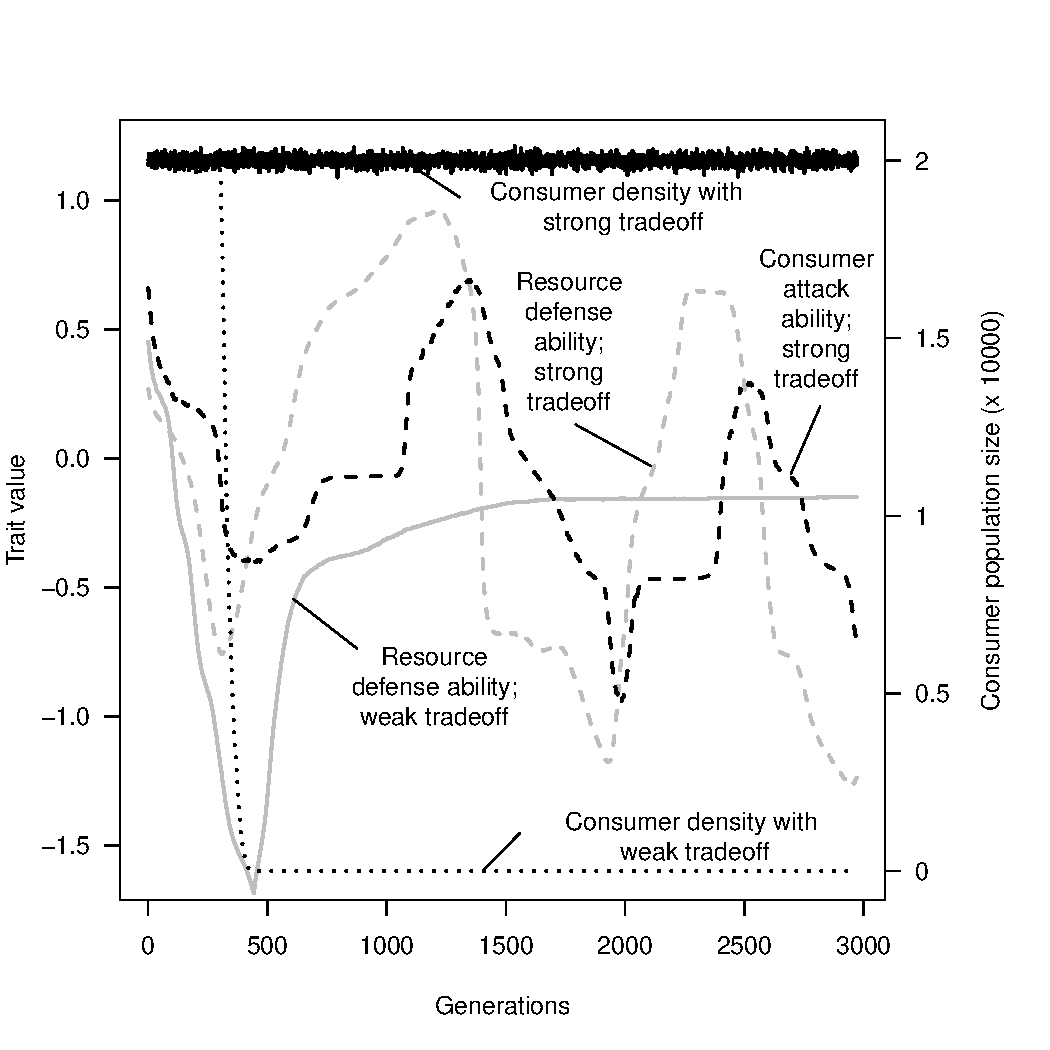
\includegraphics[width=\linewidth] {SupplementaryFigures/FigS3A.pdf}\quad
	\caption*{(A)}        
	\vspace{-1\baselineskip}

	\end{subfigure}
   \begin{subfigure}[b]{0.49\textwidth}
    \centering
   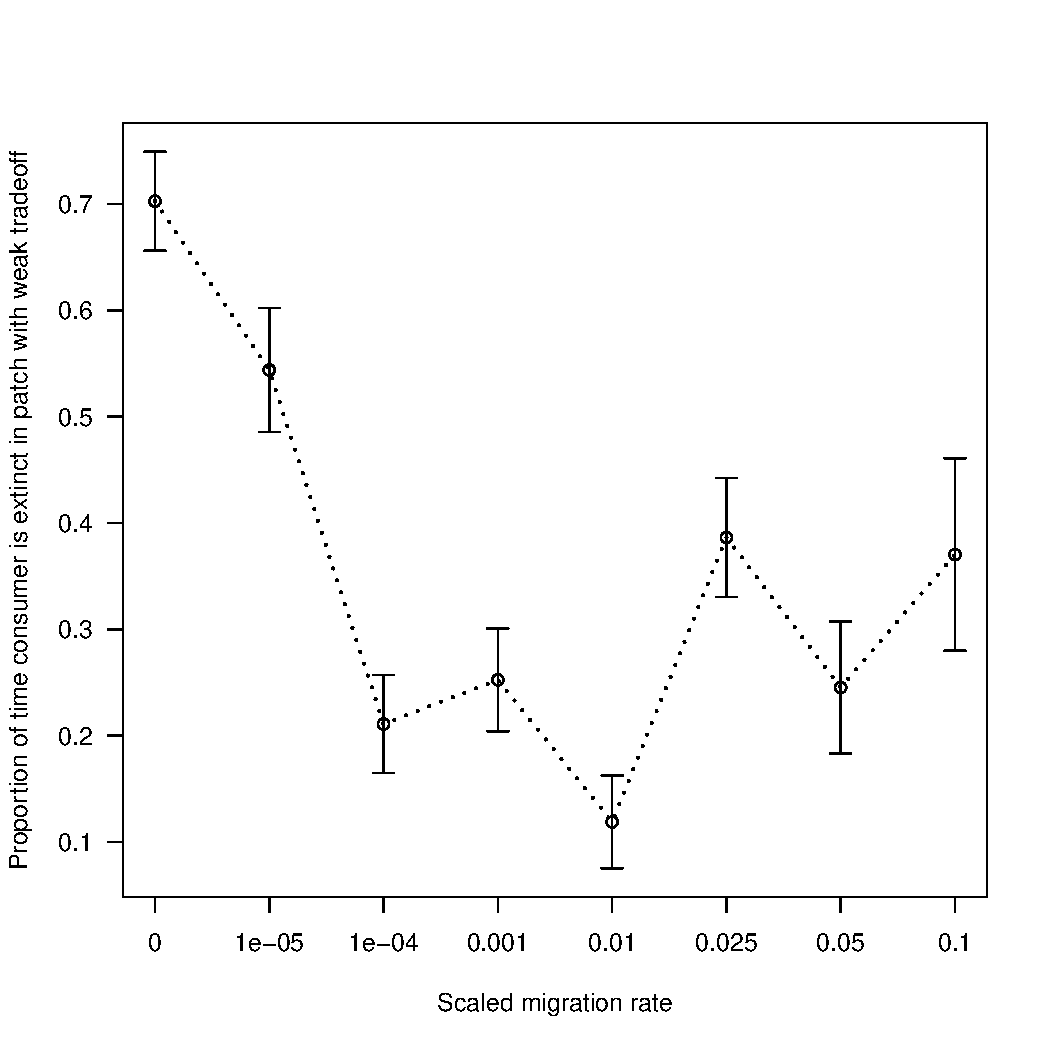
\includegraphics[width=\linewidth] {SupplementaryFigures/FigS3B.pdf}\quad
	\caption*{(B)}
        \vspace{-1\baselineskip}
  	\end{subfigure}
\caption*{}

\end{figure}
Supplementary Figure S3. (A) Coevolutionary dynamics in a consumer-resource community without migration. The traits affecting inter-specific interactions for the resource are subject to a pleiotropic constraint $\rho$ on fitness, which is modeled as reducing their per-capita fecundity following interactions with intra-specifics (i.e., their competitive ability) depending on how much the resource defense ability trait deviates from zero. The consumer, by contrast, is assumed to face no such constraint. Consumer-resource coevolution is therefore possible only in environments where the tradeoff faced by the resource is strong (black dashed line). (B) The effect of varying the scaled migration rate on consumer persistence, i.e., the proportion of time in which the consumer population is extinct, in the patch with relatively weak constraints on the resource defense trait. A biased island dispersal model is used, in which a proportion $\pi$ of migrants from each patch ultimately return to their patch of origin. Thus, the values on the abscissa in panel (B) represent the effective migration rate scaled by the propensity of individuals to attempt to leave their home patch. Error bars reflect the standard deviation across 15 replicate simulations. 


\end{document} 
